\section{Algorithm}\label{sec:optimization}

\comments{
Assuming every face in the carton model is rigid, which means the interior angle in each plane stays the same.  
%
Furthermore, planes are connected by hinges at the boundary of patches, and the planar layout has its front and back.}

In this section, we explain our algorithm in detail. 
Initially, assume that the 2D layout $L$ lies on the $XOZ$ plane, so that each vertex $\mathbf{v}_i=(x_i,y_i,z_i)$ in $V$ has $z_i=0$. 
Each face in $F$ has a normal $\mathbf{n}_i=(0,0,1)^T$.
%
In the first step of our algorithm, our system automatically computes the normal of the desired 3D carton based simple rules of orthogonality and parallelism.
In the second step, the carton shape is refined based on a set of possible geometric constraints.



%\cxj{re-write this section. Describe clearly about the parameters, the objective, and methods. }
%In this section we explain the reason why using a specific angle to each fold edge, and constructing our initialized model. 

A general process for humans to fold a carton starts from folding each edge by a rough angle and then connecting close vertexes to obtain a box-like shape. 
Naturally, we first fold the 2D layout by assigning a rotation angle to each pair of adjacent faces to get a rough shape, instead of directly computing the vertex coordinates.
%The basic idea is to interpret the folded state of a box as a series of rotation angles along each edge, and by setting specific value of angles which is $\pi/2$, we can have a rough model to assist the later optimization.
%	
Observed from existing data in the Internet, most of the traditional cartons are cuboid for holding files or delivering daily supplies. 
Although there is a recent trend to design more complicated layouts to attract consumers, the shape of these unusual cartons is similar to boxes as their functions are still packaging commodity. 
%
Therefore, we choose $\pi/2$ as the initial value of the rotation angle to each folding edge. 
%
First, a face graph of a layout is constructed, as shown in Figure~\ref{fig:midresult} (a).
Each face is a node, and there is an edge between two faces if they are connected by a folding edge.
%
The faces in the 2D layout are recursively folded in a breadth-first manner.
Starting from the face with the maximal area, our system folds all its adjacent faces by rotating them around their connecting edge by $\pi/2$, and then continues to others. 
Figure~\ref{fig:midresult} illustrates the folding process of a cuboid carton. 

\begin{figure}[ht]
	\centering
	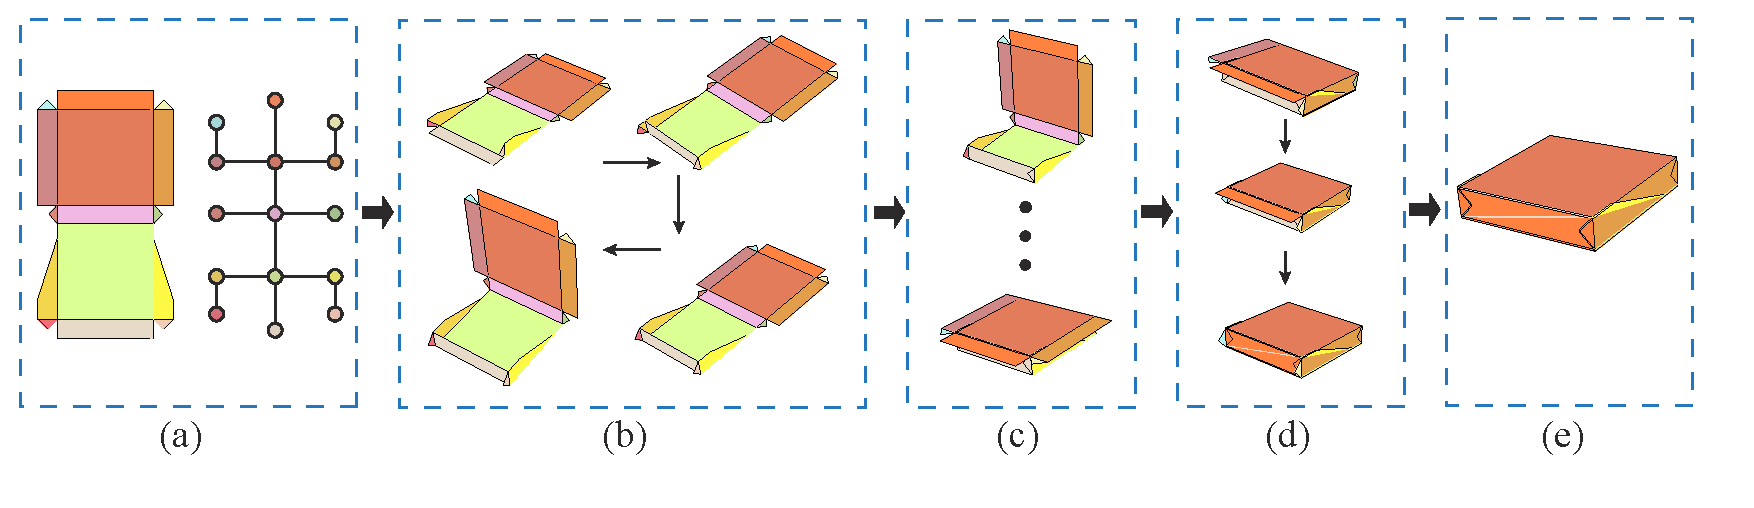
\includegraphics[width=0.9\textwidth]{images/midresult}
	\caption{A rough 3D shape is obtained by folding each face by $\pi/2$ in the 2D layout (a) in a breadth-first manner, starting from the face with the maximal area. (b), (c), (d) and (e) are the different folding stages in the initialization step.}
	\label{fig:midresult}
\end{figure}


{\color{blue}{The following two figures}} shows a group of results generated by simply folding faces by $\pi/2$.
Traditional cartons in cuboid shapes could reach an ideal state, as Figure~\ref{fig:initial-automatic} shows.
However, many complicated designs still need refinement, such as the four examples in Figure~\ref{fig:initial-need-improvement}. 
Take the hexagonal box as an example, the 3D model can be improved by simply snapping the small paste faces to its nearby faces. %
%
As a result, we provide an suggestive interface by automatically detecting potential geometric modifications in the rough carton shape for users to explore.
%interactively allow users to add these constrains into our system and optimize to a desired model, as described in the following section.

\begin{figure}
	\centering
	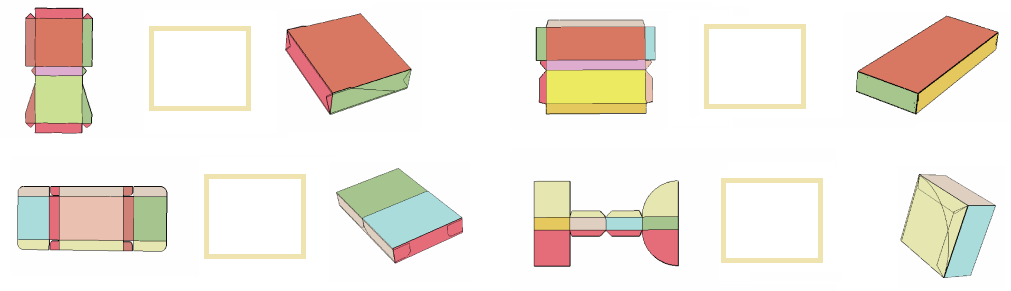
\includegraphics[width=0.9\textwidth]{images/initial-auto.png}
	\caption{Four examples of carton models that can be fully automatically generated from 2D layouts by folding each edge with a fixed angle $\pi/2$. }
	\label{fig:initial-automatic}
\end{figure}


\begin{figure}
	\centering
	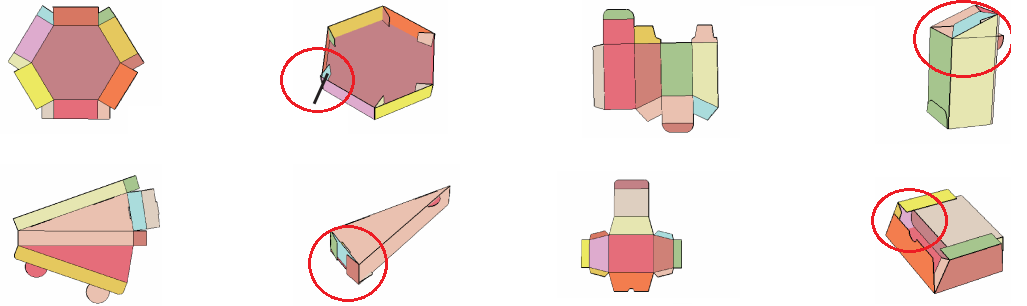
\includegraphics[width=0.9\textwidth]{images/initial-improve.png}
	\caption{Four examples of the carton models that need shape improvement. While the shapes are not cuboid, using a fixed angle $\pi/2$ leads to non-closed shape and loose structure. }
	\label{fig:initial-need-improvement}
\end{figure}
%%%%%%%%%%%%%%%%%%%%%%%%%%%%%%%%%%%%%%%%%%%%%%%%%%%%%%%%%%%%%%%%%%%%%


\subsection{Shape Constrain}
After initialization, there is still a need to refine the results that have not folded into pleasing results. The main idea is to prescribe the shape constrains by a set of vertices of the polymesh. Moreover, with the extra information acquired from user interaction, we can finally construct the ideal 3D realization compared to the ground truth. As you can see, the coordinate of vertices are chosen as our input instead of fold angles on edges, the reason is that constrains represented by vertices are simpler and more intuitive than angles, and we can implement the algorithm introduced by Bouaziz et al. easily~\cite{Bouaziz:2012:SSD:2346796.2346802}.

We now introduce the constrains used in our construction method:

\noindent
\textbf{Edge Constrain} For each edge $\{e_j\}_{j=1...M}$, we have its start point $\mathbf{v}_{js}$ and end point $\mathbf{v}_{jt}$, then we have 
\begin{equation}
||\mathbf{v}_{js} - \mathbf{v}_{jt}||^2 = ||\mathbf{\hat{v}}_{js} - \mathbf{\hat{v}}_{jt}||^2,
\label{equ:edge}
\end{equation}
to ensure that the length of each edge stays the same.

\noindent
\textbf{Coplane Constrain} For each plane $\{p_k\}_{k=1 \dots P}$ and its normal $\mathbf{n}_k$, each line connected by two points $\mathbf{v}_{ka}, \mathbf{v}_{kb}$ on the plane is perpendicular to the normal.
\begin{equation}
\mathbf{n}_k \cdot (\mathbf{v}_{ka} - \mathbf{v}_{kb}) = 0.
\label{equ:coplane}
\end{equation}

\noindent
\textbf{Plane Constrain} For each plane $\{p_k\}_{k=1 \dots P}$, the length of each line connected by two non-adjacent points $\mathbf{v}_{ka}, \mathbf{v}_{kb}$ on the plane remains the same, so that the shape of each plane keeps unchanged.
\begin{equation}
||\mathbf{v}_{ka} - \mathbf{v}_{kb}||^2 = ||\hat{\mathbf{v}}_{ka} - \hat{\mathbf{v}}_{kb}||^2.
\label{equ:plane}
\end{equation}

The information acquired from user interaction will add enough constrains to solve the optimization problem, and one of the interaction is to choose the right given suggestion including points needed to be merged together. As for the point information, the constrains can be written like:

\noindent
\textbf{Point Constrain} 
\begin{equation}
\mathbf{v}_p - \mathbf{v}_q = 0,
\label{equ:point}
\end{equation}
if these two points $\mathbf{v}_p$, $\mathbf{v}_q$ need to be moved into the same place.

When the above constrains still lead to an ill posed problem, a soft constrain will be introduced:

\noindent
\textbf{Irrelevant Point Constrain} Points $\{\mathbf{v}_i\}$ which are not in the same plane with $\mathbf{v}_p$ or $\mathbf{v}_q$, should be near the original location, and this constrain just take a light weight $w$, which is set 0.001 in our experiment. 
\begin{equation}
\mathbf{v}_i - \mathbf{\hat{v}}_i = 0.
\label{equ:irrelevant}
\end{equation}

Figure~\ref{fig:constrain} illustrates the necessity of basic three constrains.

\begin{figure}
	\centering
	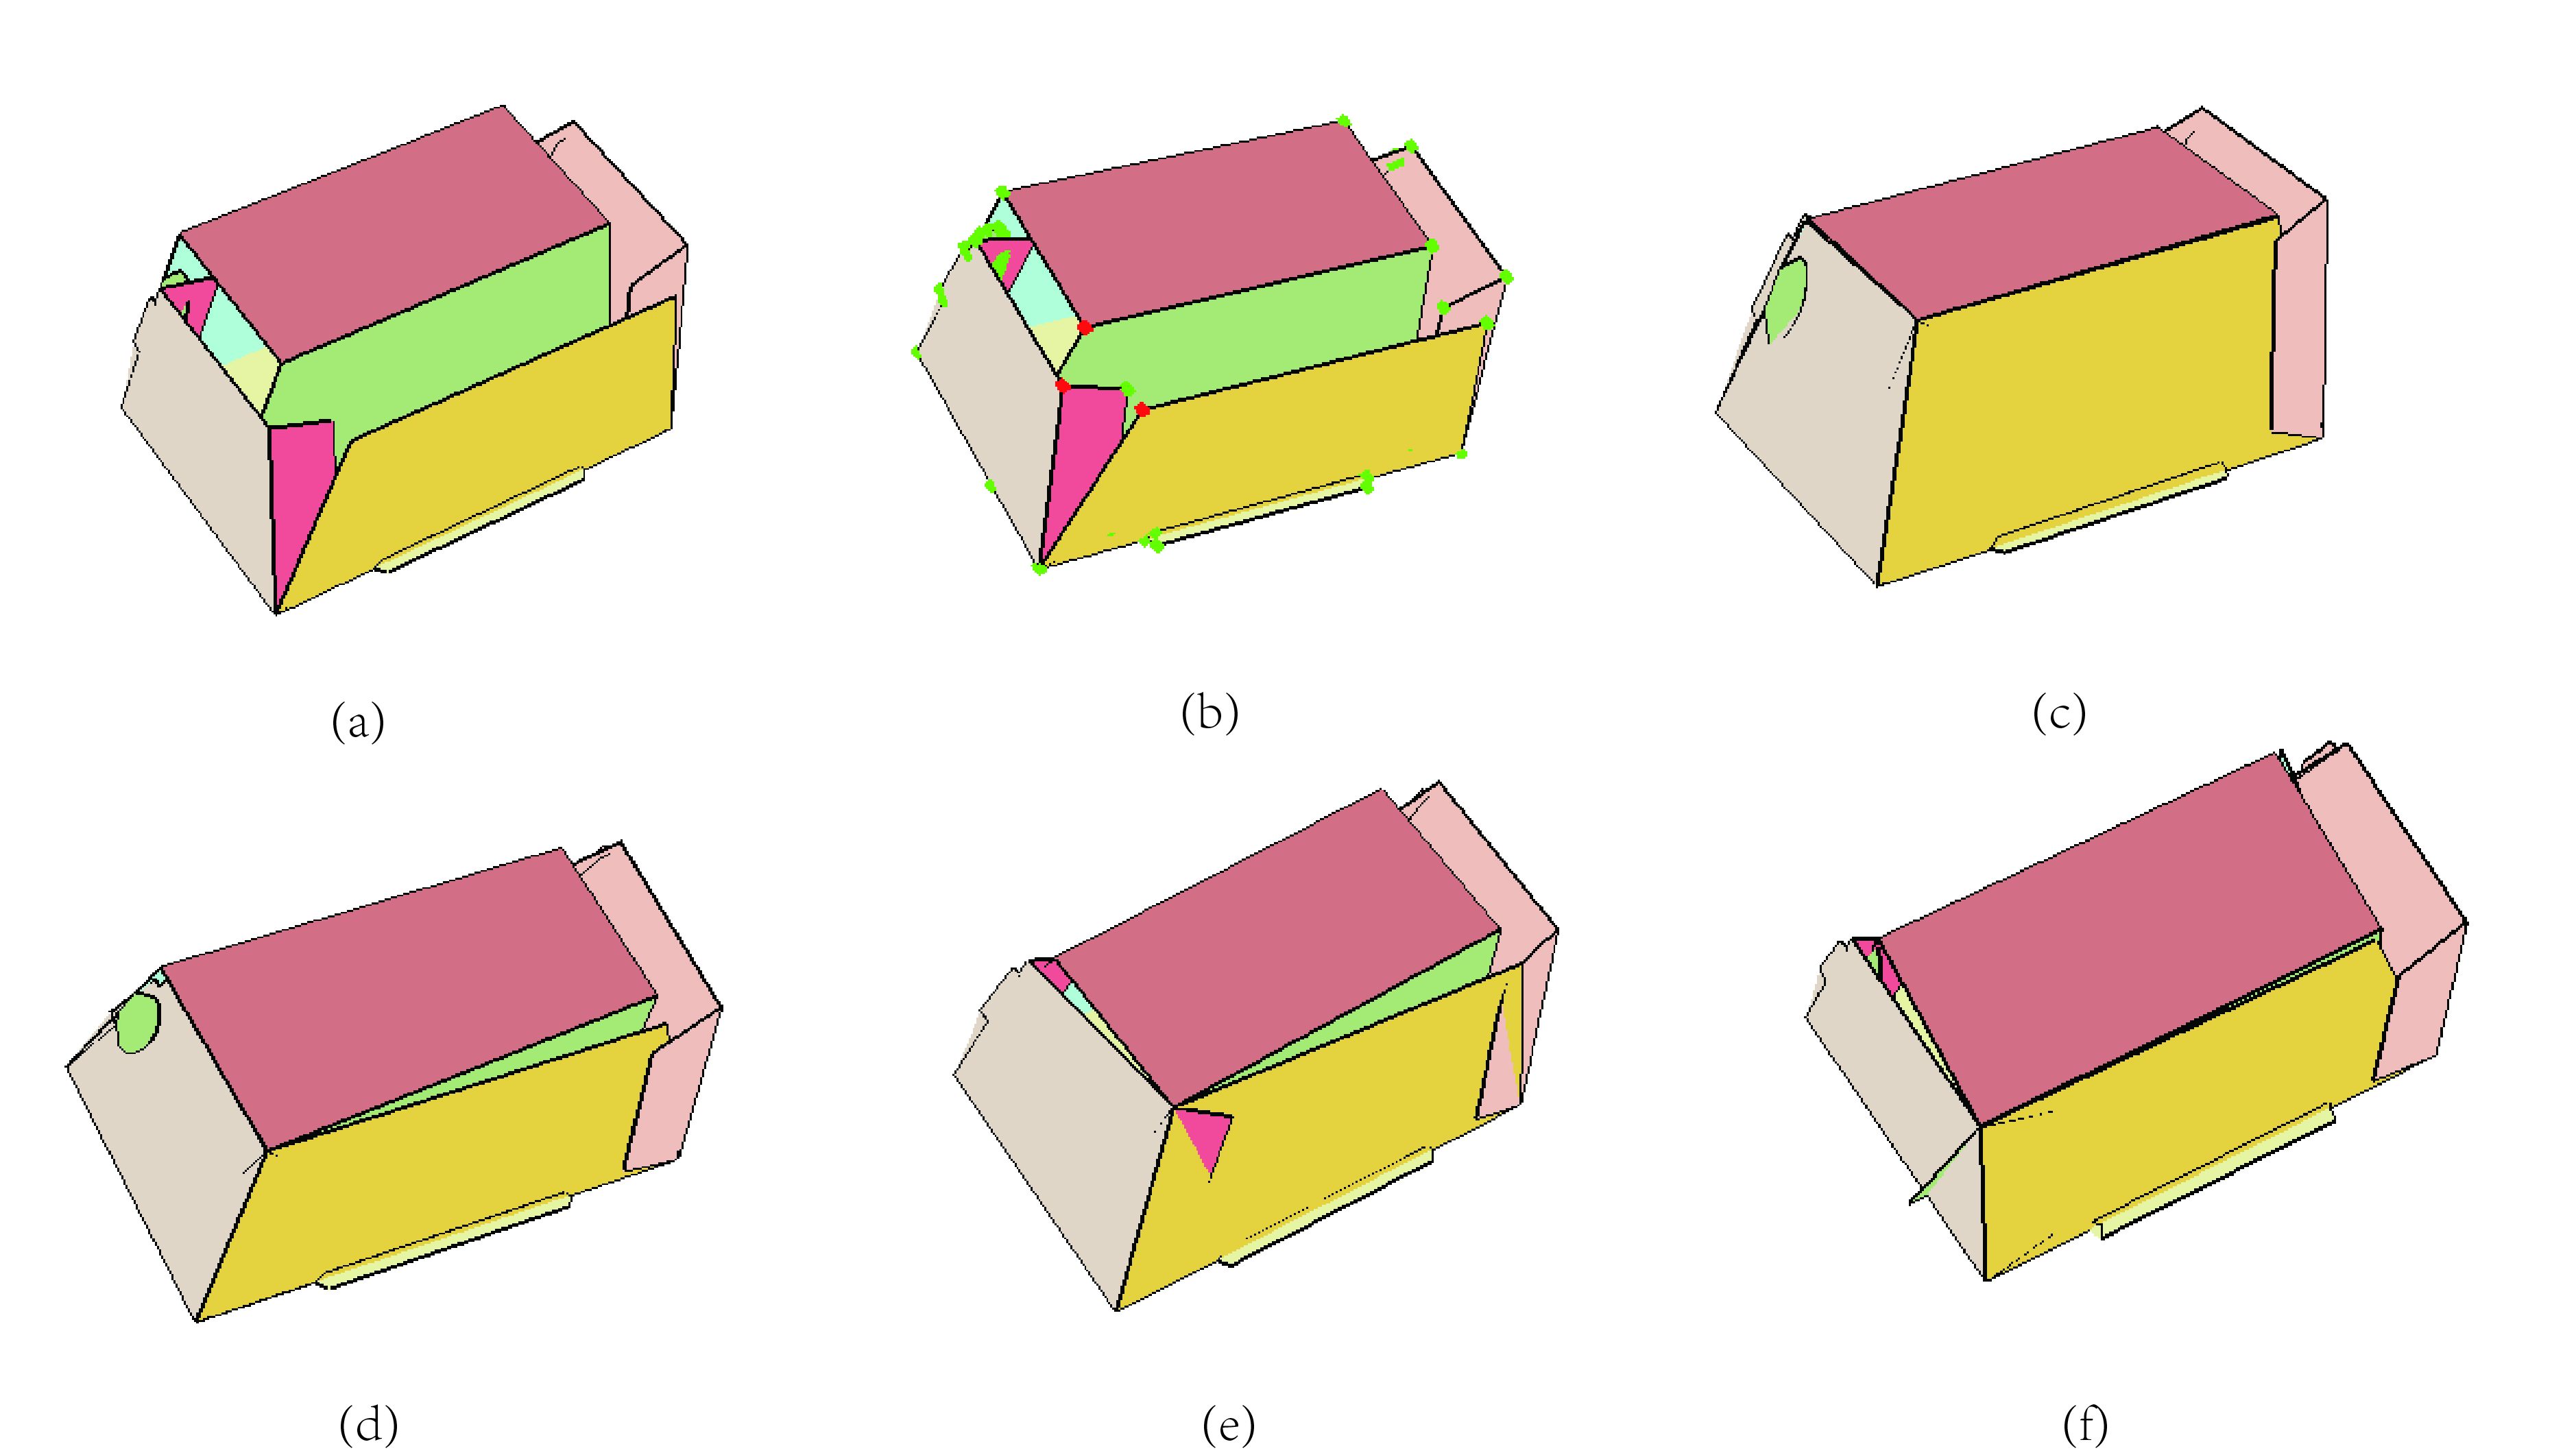
\includegraphics[width=0.9\textwidth]{images/constrain.jpg}
	\caption{Given an initial state~(a), by choosing three points marked in red~(b) that need to be relocated together, basic three shape constrains can lead to the optimization result~(c). The bottom three are the results optimized lack of edge constrain, coplane constrain and plane constrain separately, compared to~(c), the results can not keep the basic shape well.}
	\label{fig:constrain}
\end{figure}


\subsection{Aided Detection}

While the initial 3D model with simple angle folding provides a rough idea about the carton shape, our system could automatically detect a group of possible shape constraints to form the final 3D model, such as vertex merging, shape symmetry, and so on. 
%
These guiding operations are provided to the user at bottom of the user interface, for the user to quickly select and explore the carton shapes.

%
In order to asist users construct the final carton interactively, we also provide symmetry detection and merging points detection to improve the efficiency of constructing models .

\noindent
\textbf{merging points detection} Consider the initialization results can represent the ideal model partly, the disadjacent vertices that have one edge with same length can be regarded as targets that need to be located in the same place if their Euclidean distance is below a certain threshold.

\noindent
\textbf{symmetry detection} On account of the simplicity of the carton shape, the vertices that have same length set of incident edges can be regarded as symmetric pair. While users select vertices that need to be merged together, symmetry detection can reduce repetitive work by giving users suggestions of symmetric vertices.